\hspace{5mm} Machine learning consists of the following four classes: i) Supervised learning, ii) Unsupervised learning, iii) Semi-supervised learning, iv) Reinforcement learning.  Supervised learning is fitting a model to a set of labeled data provided by a subject matter expert.  Subsequently, unsupervised learning is used on unlabeled data sets.  The objective of unsupervised learning is to explore the data and identify hidden features. Semi-supervised learning combines the strengths of supervised and unsupervised learning, and is especially useful \cite{machine_learning}.  Often times, industrial data will be partially labelled due to the time and cost associated with data labelling.  For supervised and unsupervised learning, only the labeled and unlabeled data can be used, respectively.  However, all data can be used in semi-supervised learning which allows for maximized data efficiency and increased model performance. Finally, reinforcement learning is a goal-directed learning from interactions with the environment \cite{sutton}. It is used to find the optimal policy (i.e., optimal input trajectory) through guidance from an internal scalar reward (feedback).  


\section{Introduction to Reinforcement Learning}

In general terms, reinforcement learning is simply the learning an agent experiences through interactions with the environment.  For added intuition, Figure \ref{fig: simple_rl} shows the generic information flow of reinforcement learning.  An agent exists in an environment, and learns through interactions.  First, the agent observes some states, $x_t \in X$, from the environment (some states may be unobservable).  Given $x_t$, the agent performs some actions, $u_t \in U$ and receives a scalar reward signal, $r \in \mathbb{R}$.  Finally, the environment will transition to a new state, $x_{t+1}$, given probability $T(x_{t+1}, r | x, u)$.

\begin{figure}[h]
    \centering
    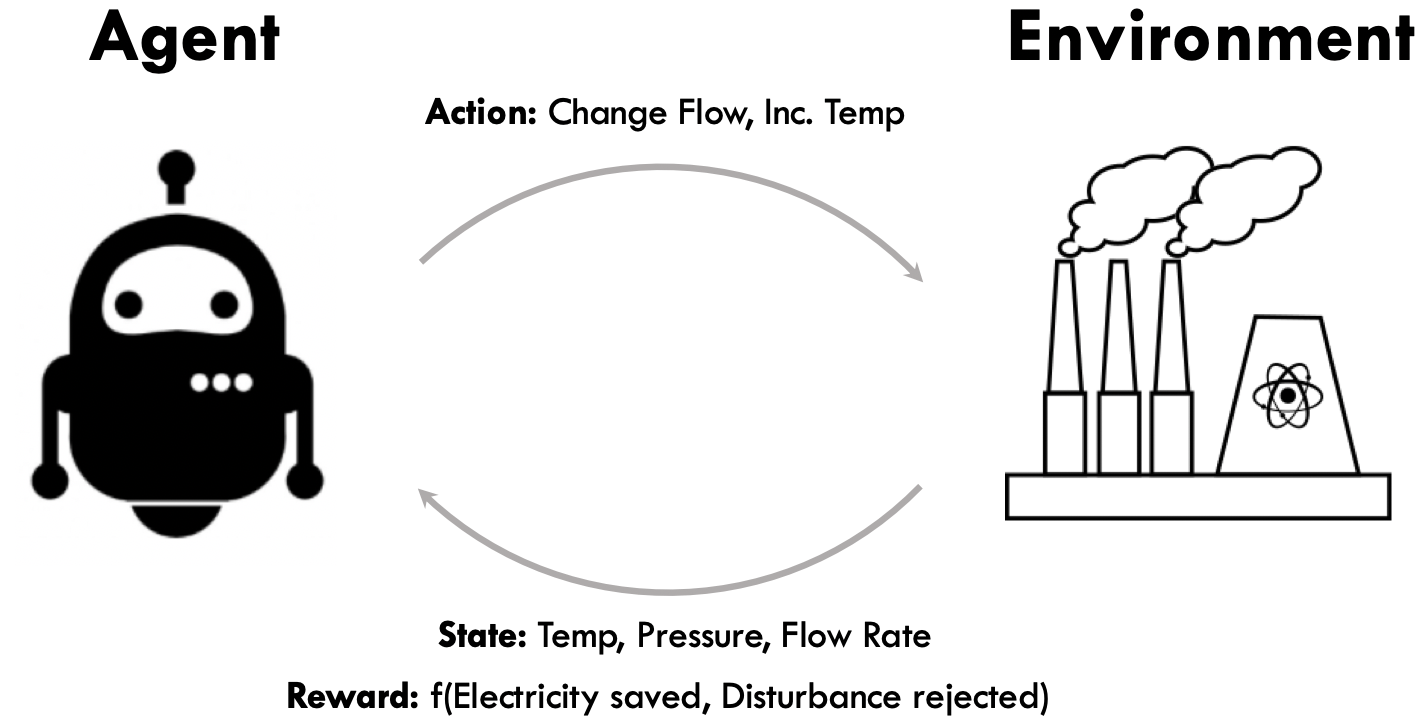
\includegraphics[scale=0.5]{images/RL.png}
    \caption{Basic setup of reinforcement learning where an agent interacts with the environment}
    \label{fig: simple_rl}

\end{figure}

Reinforcement learning consists of the following four elements:

\begin{itemize}
    \item Policy, $\pi$
    \item Reward, $R$
    \item Value Function, V(s)
    \item Model (optional), $\dot{x} = Ax + Bu$
\end{itemize}

The policy, $\pi$, of reinforcement learning is a direct mapping from $S \rightarrow A$.  To find the optimal policy, $\pi^*$, the agent is guided by an immediate scalar reward for each interaction (also called \textit{episode}). Policies that result in higher rewards are more likely to happen in the future, mutatis mutandis.  However, reinforcement learning is concerned with the long term success rather than immediate pleasure. Often times, long term success require short term sacrifice.  Thus, the value function, $V^{\pi}(s)$, is used to describe the long term expected reward under each policy.

Exploration vs exploit
model based vs model free

\subsection{Reinforcement Learning's Uniqueness}
Reinforcement learning is a unique class of machine learning.  An ideal supervised learning model can only be as good as the subject matter expert providing the labels to the data set, which may not be 100\%.  For example, in a complex control task, the control law is usually highly non-linear. Control experts can try to provide control strategies for such systems, but optimality may not be guaranteed for highly non-linear systems. Also, supervised learning is used to generalize responses for occurrences not present in the data \cite{sutton}.  Reinforcement learning works by directly interacting with the environment \textit{without labels}. Through adequate exploration, reinforcement learning will identify peculiar features to optimally control such problems [citation required].  Reinforcement learning is \textit{similar} to unsupervised learning in terms of identifying hidden structures within the environment.  However, reinforcement learning tries to maximize an internal scalar "reward" signal, rather than purely data mining.

Evolutionary methods, a family of optimization algorithms such as genetic algorithm, is most similar to reinforcement learning.  For a control problem, such methods can apply multiple static policies for different operating regimes \cite{sutton}.  Policy search is conducted by first initiating $k$ random input trajectories of length $N$, generating input matrix $\mathbb{U}_{[k, N]} \in \pi$.  Subsequently, the loss, $J_U$, of each $U$ is calculated based on the objective function.  Input trajectories with the lowest loss move onto the next generation and generates new pseudo-random input trajectories.  This process is repeated until optimal policy, $\pi^*$ is found for each operating regime \cite{ga_for_control}.

Evolutionary methods work well when the policy space is sufficiently small, easy to find, or a lot of time is available for optimization.  The biggest advantage of such methods compared to reinforcement learning is that the whole state does not need to be known.  However, such methods does not capture the reinforcement learning fundamentals of mapping $S \rightarrow A$.  Unlike evolutionary methods, reinforcement learning keeps memory of each indvidual interaction making it a more data efficient approach \cite{sutton}.


Exploration vs exploit
model based vs model free





\subsection{Value-Iteration}
\subsection{Policy-Iteration}
\subsection{Expected Returns for Different MDPs}
\subsection{Adaptation to Non-Stationary Problems}

%%%%%%%%%%%%%%%%%%%%%%%%%%%%% End Section Intro to RL %%%%%%%%%%%%%%%%%%%%%%%%%%%%%%%%%%%%%%%


%%%%%%%%%%%%%%%%%%%%%%%%%%%%% Begin Section Tabular RL %%%%%%%%%%%%%%%%%%%%%%%%%%%%%%%%%%%%%%

\section{Tabular Reinforcement Learning}
\subsection{Problem Setup}
\subsection{Action Selection}
\subsection{Reward Functions}
\subsection{Exploration in Tabular Reinforcement Learning}

%%%%%%%%%%%%%%%%%%%%%%%%%%%%% End Section Tabular RL %%%%%%%%%%%%%%%%%%%%%%%%%%%%%%%%%%%%%%%

%%%%%%%%%%%%%%%%%%%%%%% Begin Section Function Approximation %%%%%%%%%%%%%%%%%%%%%%%%%%%%%%%

\section{Function Approximation}
\subsection{Introduction to Function Approximations}
\subsection{Neural Network Basics}
\subsubsection{Neural Network Initialization}
\subsubsection{Gradient Descent Updating}
\subsubsection{Mini-batch Gradient Descent}
\subsubsection{Batch Normalization}
\subsubsection{Regularizations}

%%%%%%%%%%%%%%%%%%%%%%%%% End Section Function Approximation %%%%%%%%%%%%%%%%%%%%%%%%%%%%%%%


%%%%%%%%%%%%%%%%%%%%%%%%%%%%%%%%% Begin Section DDPG %%%%%%%%%%%%%%%%%%%%%%%%%%%%%%%%%%%%%%%

\section{Deep Deterministic Policy Gradient}
\subsection{Actor-Critic Intuition}
\subsection{Actor - Deterministic Policy Gradient}
\subsection{Critic - Deep Q-learning}

\newpage

\subsection{Exploration in DDPG}
\subsubsection{White Exploratory Noise}
\subsubsection{Ornstein-Uhlenbeck Exploratory Noise}
\subsection{Stabilization of Training}
\subsubsection{Experience Replay}
\subsubsection{Target Network}
\subsubsection{Adaptive Batch Gradient Descent}
\subsubsection{Reward Clipping}
\subsection{Input and State Constraints}
\subsection{Training Algorithm}

%%%%%%%%%%%%%%%%%%%%%%%%%%%%%%%%%% End Section DDPG %%%%%%%%%%%%%%%%%%%%%%%%%%%%%%%%%%%%%%%%
